\documentclass[12pt]{article}
\usepackage{graphicx}
\usepackage{adjustbox}
\usepackage{tikz}
\usetikzlibrary{automata, arrows, positioning, fit, calc}

\begin{document}

% Distributed RL Architecture
\resizebox{\textwidth}{!}{%
	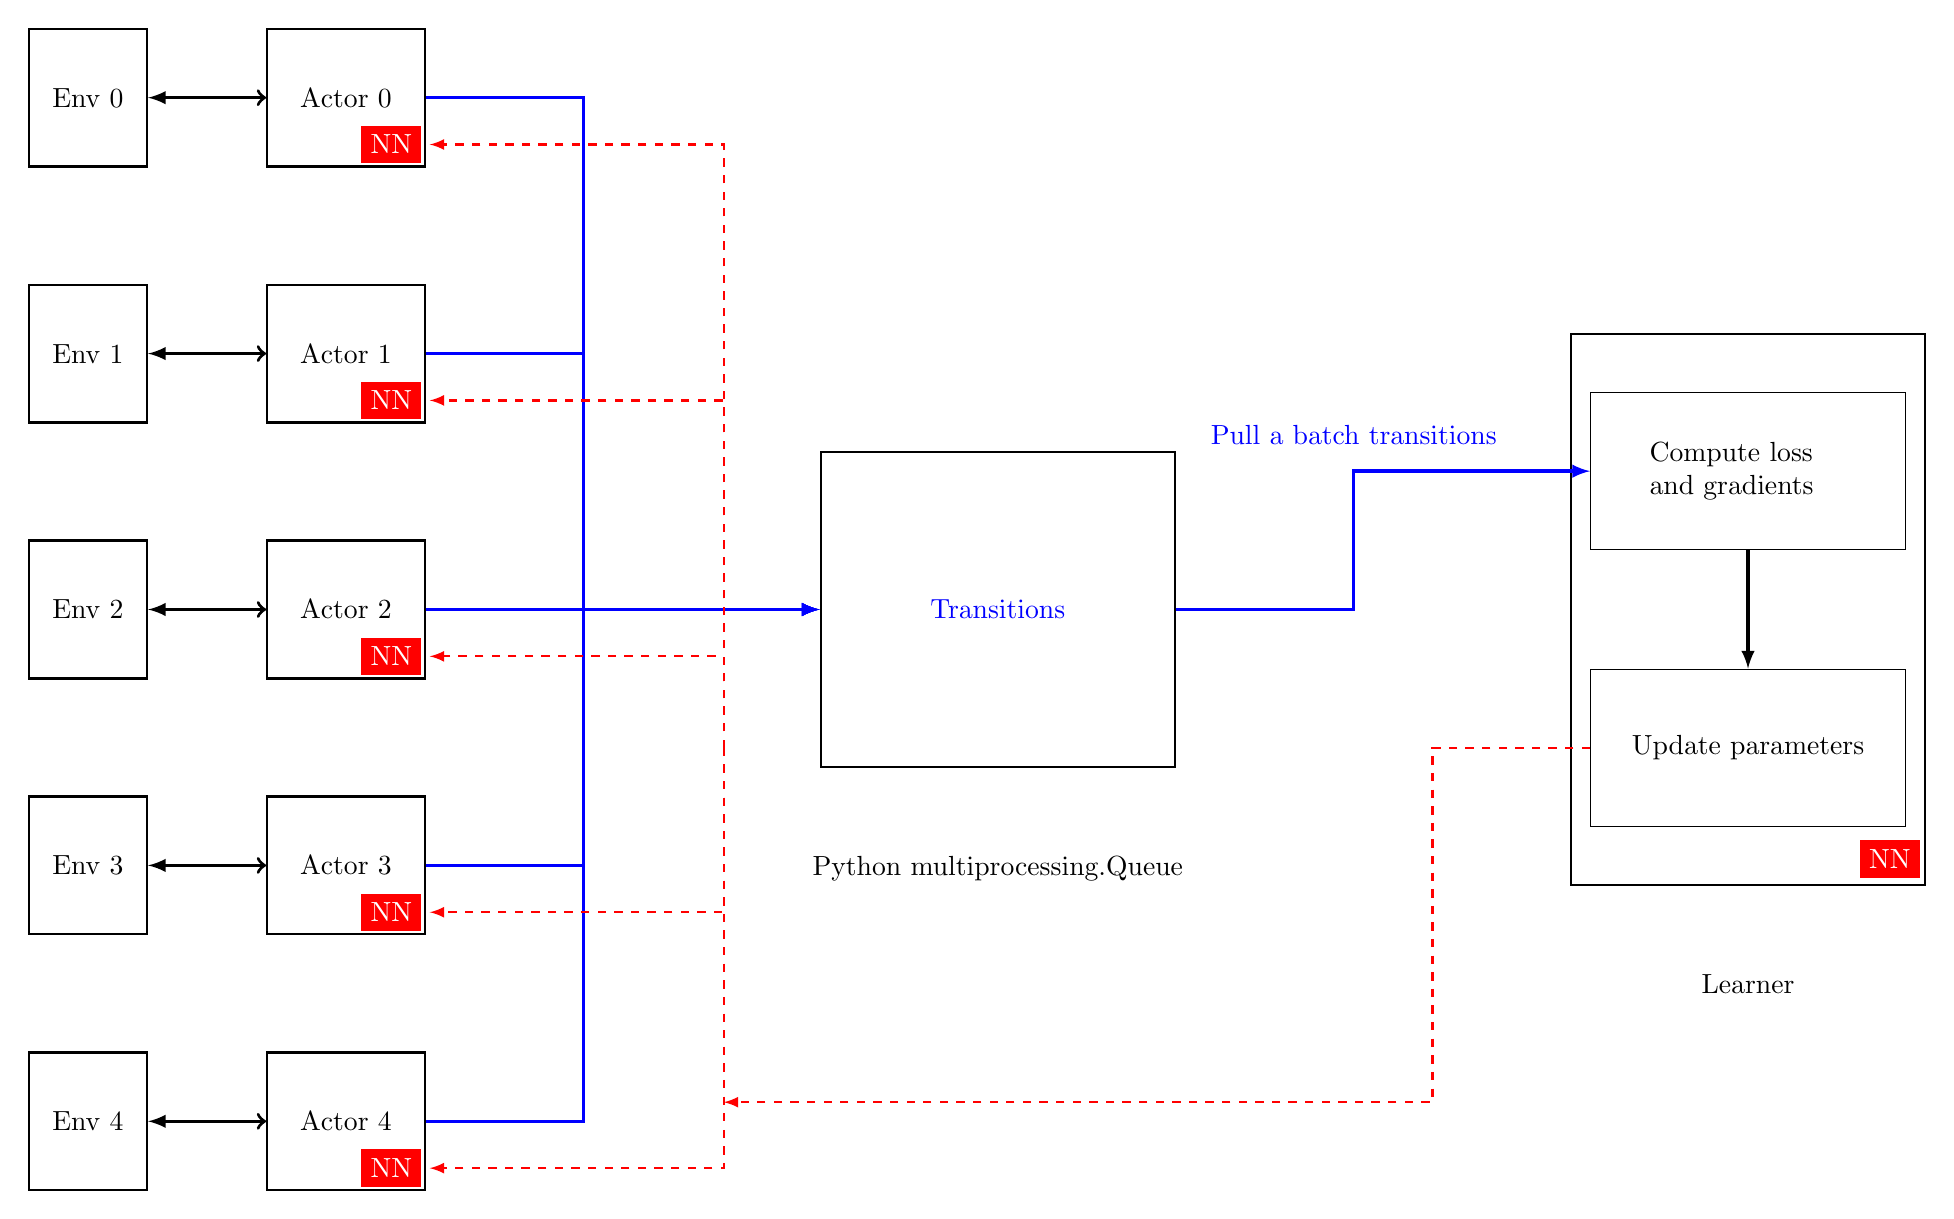
\begin{tikzpicture}[node distance=3.5cm]
		\tikzstyle{actor} = [rectangle, draw=black, thick, minimum size=2cm, minimum height=1.75cm, text width=1.5cm, inner sep=0, align=center]
		\tikzstyle{env} = [rectangle, draw=black, thick, minimum size=1.5cm, minimum height=1.75cm, text width=1.5cm, inner sep=0, align=center]
		\tikzstyle{learner} = [rectangle, draw=black, thick, minimum size=4.5cm, minimum height=6cm, text width=2.25cm, inner sep=0, align=center]

		\tikzstyle{directed_line} = [-latex, very thick,]
		\tikzstyle{bydirec_line} = [<-latex, very thick]
		\tikzstyle{transition_line} = [-latex, very thick, blue]
		\tikzstyle{param_line} = [-latex, dashed, thick, red]

		% Actors
		\foreach \i in {0,1,2,3,4} {
				\node[actor](actor_\i) at (0, -\i*3.25) {Actor \i};
				\node[env, left=1.5cm of actor_\i](env_\i){Env \i};
				\path[bydirec_line] (actor_\i) edge (env_\i);
				\node[rectangle, color=white, fill=red](actor_\i_nn) at ($(actor_\i.south east)+(-0.5mm,0.5mm)$) [anchor=south east] {NN};
			};

		% Queue
		\node[rectangle, text=blue, draw=black, thick, minimum size=4.5cm, minimum height=4cm, right=5cm of actor_2](queue)
		{Transitions};
		\node[below=1cm of queue.south]{Python multiprocessing.Queue};

		% Learner
		\node[rectangle, draw=black, thick, minimum size=4.5cm, minimum height=7cm, right=5cm of queue](learner){} node[below=1cm of learner.south]{Learner};

		\node[rectangle, draw, minimum size=4cm, minimum height=2cm, below=0.75cm of learner.north, text width=2.5cm](learner_loss){Compute loss and gradients};
		\node[rectangle, draw, minimum size=4cm, minimum height=2cm, above=0.75cm of learner.south](learner_update){Update parameters};
		\node[rectangle, color=white, fill=red] at ($(learner.south east)+(-0.75mm,1mm)$) [anchor=south east] {NN};

		\path[directed_line] (learner_loss) edge (learner_update);

		% Add save new transition edges
		\foreach \i in {0,1,2,3,4} {
				\draw[transition_line] (actor_\i.east) -| ($(queue.west)+(-3cm,0cm)$) |- (queue.west);
			};

		% Draw perpendicular line from transition to leaner
		\draw[transition_line](queue.east) -| ($(learner_loss.west)+(-3cm, 0cm)$) |- (learner_loss.west) node[midway, above=2mm]{Pull a batch transitions};

		% Add update network path
		\draw[param_line] (learner_update.west) |- ($(learner_update.west)+(-2cm,0cm)$) |- ($(learner_update.west)+(-11cm,-4.5cm)$);
		\foreach \i in {0,1,2,3,4} {
			\draw[param_line] ($(learner_update.west)+(-11cm,0cm)$) |- ($(actor_\i_nn.east)+(1mm,0cm)$);
		};

	\end{tikzpicture}
}

\end{document}
